\section{Durchführung}
\label{sec:Durchführung}

Im Versuch wird der Depolarisationsstrom von mit Strontium dotiertem Kaliumbromid (KBr) in Abhängigkeit
von der Temperatur für zwei verschiedene Heizraten gemessen. Dazu steht die in
Abbildung \ref{fig:aufbau} dargestellte Apparatur zur Verfügung.

\begin{figure}
  \centering
  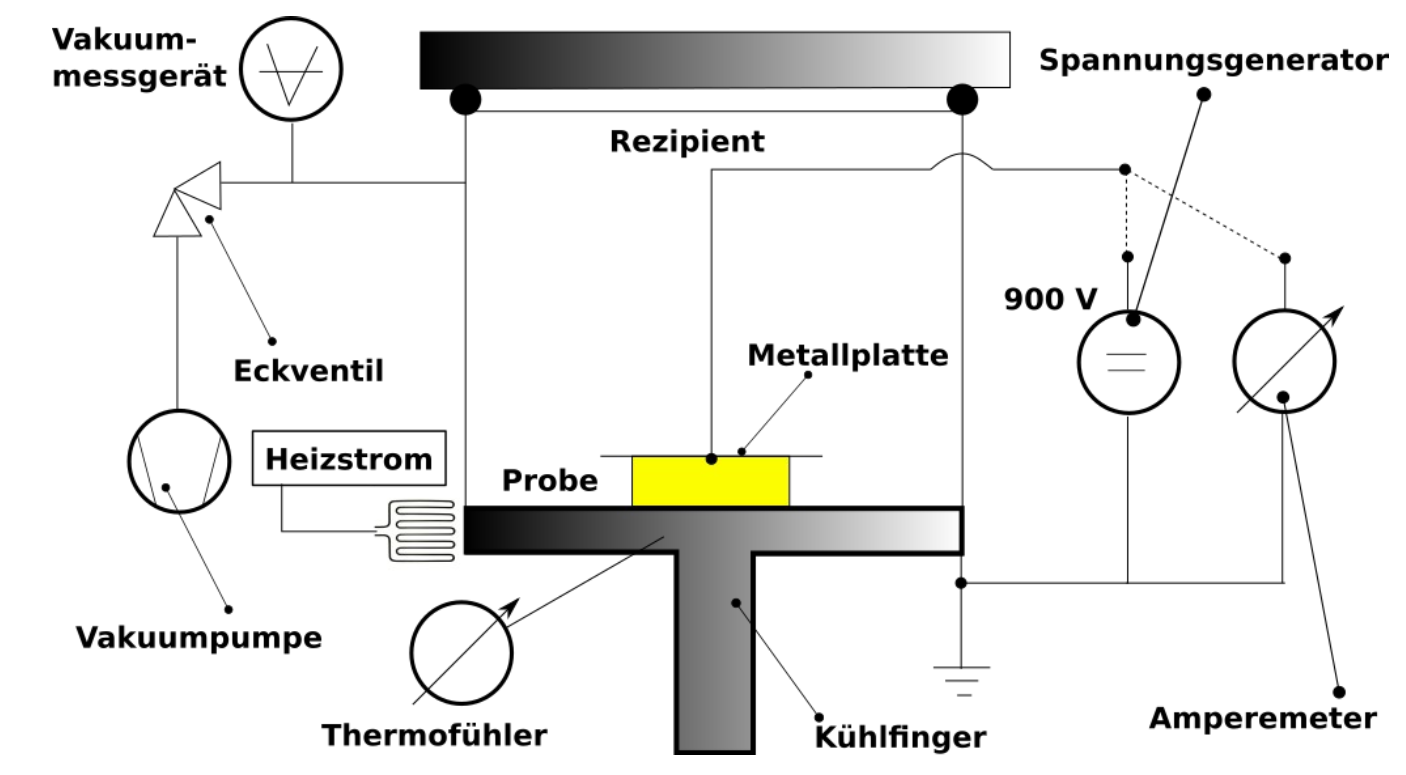
\includegraphics[width=0.9\textwidth]{data/aufbau.png}
  \caption{Skizze des Versuchsaufbaus \cite{Versuchsanleitung}.}
  \label{fig:aufbau}
\end{figure}

Zu erkennen ist dort eine Probe, die am Boden eines Kondensators angebracht ist.
Der gesamte Kondensator befindet sich in einem Rezipienten, der während des
Versuchs evakuiert werden muss, da die Probe hygroskopisch ist. Die untere Platte
des Kondensators (und damit auch die Probe) ist mit einem Kühlfinger verbunden,
der in flüssigen Stickstoff getaucht werden und somit die Kondensatorplatte
und die Probe kühlen kann. Außerdem ist eine Heizwicklung in der Nähe der
Probe angebracht, mit der sie kontrolliert geheizt werden kann.

Bei der Durchführung des Versuchs wird nun zunächst die Probe auf etwa 50°C erwärmt
und der Kondensator wird für etwa 900\,s aufgeladen, sodass die Probe nahezu vollständig
polarisiert ist. Anschließend wird die Probe auf etwa -60°C heruntergekühlt.
Sobald die Probe diese Temperatur erreicht hat, sind die Dipole in der Probe
"eingefroren" und der Kondensator kann kurzgeschlossen werden. Daraufhin wird das
Picoamperemeter angeschlossen. Sobald ein konstanter Wert von ca. 1-2\,pA angezeigt
wird, kann mit der Messung begonnen werden. Dafür wird durch Regelung des Stroms
an der Heizwendel eine möglichst konstante Heizrate aufrechterhalten und es wird
der Strom in Abhängigkeit von der Temperatur der Probe gemessen.

Es wird eine Messreihe mit einer Heizrate von etwa 2\,K/min und eine mit einer Heizrate
von etwa 1{,}2\,K/min aufgenommen.
